\documentclass[]{beamer}
\usepackage{beamerthemesplit}
\setbeamertemplate{caption}[numbered]
\usepackage{amsmath}
\graphicspath{{/Users/edwardmcdugald/Conductivity/doc/figs/}}

\title{Simulating the Forward Problem of Magneto-Acousto-Electric Tomography}
\author{Edward McDugald}
\institute{University of Arizona}
\date{\today}
\begin{document}

\begin{frame}
  \titlepage
\end{frame}

\begin{frame}
    \frametitle{Magneto-Acousto-Electric-Tomography (MAET)- Basic Set-up}
  \begin{itemize}
      \item Biological tissue of unknown conductivity $\sigma(x)$ is placed in a conductive medium, and subjected to a magnetic field $B$.
      \item Acoustic waves with velocity $V(x,t)$ are generated with a transducer, causing movement in the tissue.
    \item A pair of electrodes measures the change in potential at the boundary.
    \item The goal is to recover $\sigma(x)$, forming a conductivity map of the tissue.
  \end{itemize}
   \end{frame}

\begin{frame}
    \frametitle{Magneto-Acousto-Electric-Tomography (MAET)- Basic Set-up}
     \centering
            \begin{figure}
            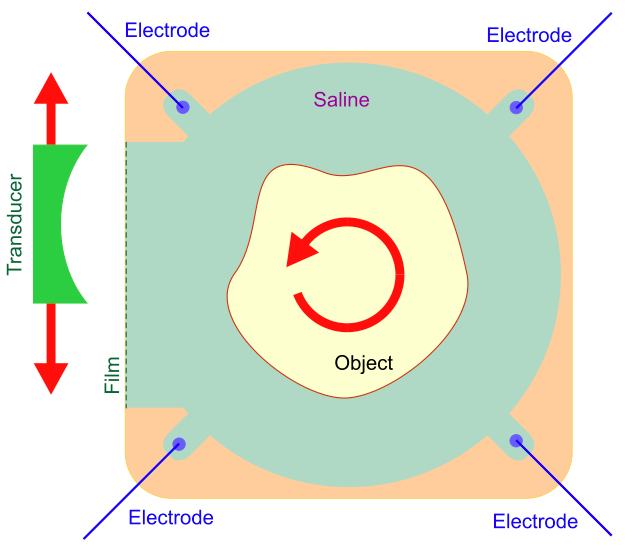
\includegraphics[scale=0.20]{MAET_Schematic.png}
            \caption{MAET Schematic}
            \end{figure}

\end{frame}


\begin{frame}
  \frametitle{Physics of MAET}
  \begin{itemize}
      \item \textbf{Lorentz Current:} Charges moving with velocity $V(x,t)$ generate Lorentz Currents
          \[
              J_L(x,t) = \sigma(x)V(t,x)\times B.
          \]
    \item \textbf{Ohmic Current:} Lorentz Force generates electric potential, $u(t,x)$, which obeys Ohm's Law. Ohmic Current is given by
        \[
            J_O(x,t) = \sigma(x)\nabla u(x,t).
        \]
    \item \textbf{Field is Divergence Free:} With total current $J = J_O + J_L$, we have
        \[
        \nabla J = 0.
        \]
    \item Therefore,
        \[
            \nabla \cdot \sigma(x)\nabla u(x,t) = -\nabla \cdot \left(\sigma(x)B \times V\right).
        \]
     \end{itemize}
 \end{frame}

 \begin{frame}
  \frametitle{Relating Measurements to Desired Quantities}
  \begin{itemize}
  \item We are able to measure differences of potential on the boundary, $M(t) = u(z_1,t)-u(z_2,t)$.
      \[
          M(t) = \int_{\Omega}J_{I}(x)\cdot B \times V(x,t)dx.
      \]
    \item Since $V(x,t)$ solves the wave equation, it satisfies
        \begin{align*}
            V(x,t) &= \frac{1}{\rho}\nabla \phi(x,t)\\
            p(x,t) &= \frac{\partial}{\partial t}\phi(x,t),
        \end{align*}
       where $\phi(x,t)$ is the velocity potential, and $p(x,t)$ is pressure.
    \item Therefore,
        \[
            M(t) = \frac{1}{\rho}B \cdot \int_{\Omega}\phi(x,t)\nabla \times J_{I}(x).
        \]
    \item $J_I(x)$ is "lead current". Does not actually exist. Will be discussed further.
\end{itemize}
\end{frame}

\begin{frame}
  \frametitle{Relating Measurements to Desired Quantities}
  \begin{itemize}
  \item In practice, we can use plane waves, $\phi(x,\tau,\omega) = \delta(x\cdot\omega-\tau)$, then
      \[
          M(\omega,\tau)=\frac{1}{\rho}B \cdot \int_{\omega}\delta(x\cdot\omega - \tau)\nabla \times J_{I}(x)dx = \frac{1}{\rho}B\cdot R(\nabla \times J_{I}(x))(\omega,\tau).
      \]
\item Therefore, the difference in potential measured by our electrodes is proportional to the Radon Transform of the curl of Lead currents.
\item The overall MAET procedure involves inverting the radon transform of the measurements to obtain curl of lead currents, from which one can obtain lead currents, and then finally the conductivity.
\end{itemize}
\end{frame}

\begin{frame}
    \frametitle{Basic Model of Lead Currents}
  \begin{itemize}
    \item $J_I(x)$ desribes the sensitivity of the system to a dipole.
    \item Lead currents arise physically by running a unit charge through the system in the absence of a magnetic field, and in the absense of acoustic waves.
\end{itemize}
 \centering
        \begin{figure}
        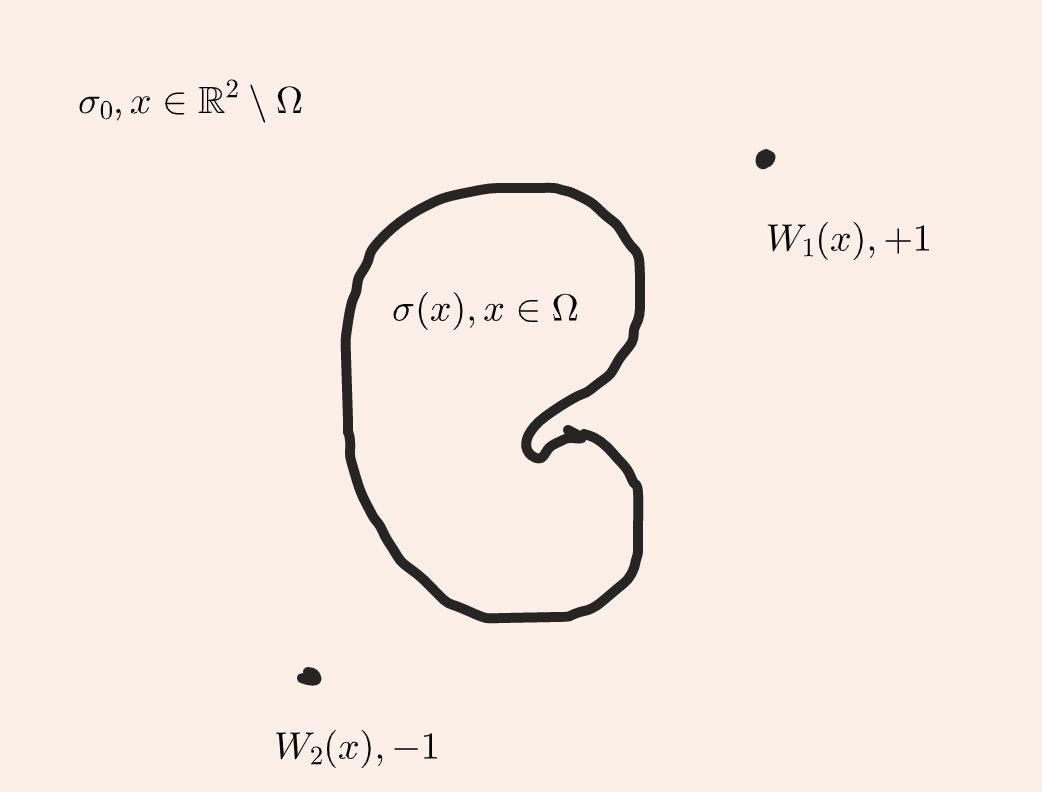
\includegraphics[scale=0.20]{lead_current_setup.png}
        \caption{Basic Setup for Lead Currents}
        \end{figure}
\end{frame}

\begin{frame}
    \frametitle{The Conductivity Equation}
  \begin{itemize}
    \item The conductivity equation takes conductivity as input, and returns electric potential.
    \item For convenience, we can split the total electric potential into smooth and non-smooth components, $u(x)$ and $w(x)$.
    \item $u(x)$ is the potential in the absence of sinks/sources, and is unknown.
    \item $w(x)$ is the potential arising from point sources, and is known.
  \item Lead current is given by
      \[
          J_I(x) = \sigma(x)\nabla(u(x)+w(x))
      \]
  \item $w(x) = -\frac{1}{\sigma_0}\sum_{j=1}^{n}W_j\Phi(x-y^{(j)})$, with $\Phi(x) = \frac{1}{2\pi}\ln(|x|)$.
\item The governing equation is the Conductivity Equation
    \[
        \nabla \cdot \sigma(x)\nabla(u(x)+w(x))=0, \quad \lim_{x \rightarrow \infty}u(x) = 0.
    \]
\end{itemize}
\end{frame}


\begin{frame}
    \frametitle{Numerical Solution - Fredholm Equation}
  \begin{itemize}
      \item The conductivity equation can be written as an integral equation of the second kind:
          \begin{multline*}
              U(x)+\frac{1}{2\pi} \Big[\frac{\partial \ln\sigma(x)}{\partial x_1}\int_{\Omega}\ln|x-y|\frac{\partial}{\partial y_1}U(y)dy\\+ \frac{\partial \ln\sigma(x)}{\partial x_2}\int_{\Omega}\ln|x-y|\frac{\partial}{\partial y_2}U(y)dy\Big]=-\nabla \ln\sigma(x)\cdot\nabla w(x).
          \end{multline*}
    \item One just needs to handle the singularities in the integrals, and apply GMRES routine.
    \item GMRES will output $U(x)=\Delta u(x)$. Potential $u(x)$ can be recovered by convolution with $\Phi(x)$.
  \end{itemize}
\end{frame}

\begin{frame}
    \frametitle{Numerical Solution - Handling Singular Kernels}
  \begin{itemize}
      \item Since we are using the Fredholm Equation of the Second kind formulation, we need to handle convolutions with a singular kernel $u(x) = \int_{\Omega}U(y)\frac{1}{2\pi}\ln|y-x|dy$
        \item Result of the convolution will satisfy the following conditions:
        \item (1) $\Delta u(x) = U(x), x \in \Omega$
        \item (2) $\Delta u(x) = 0, x \notin \Omega$.
        \item (3) $u(x)$ behaves like a Logarithm asymptotically.
        \item A function satisfying (1)-(3) will be unique.
  \end{itemize}
\end{frame}

\begin{frame}
    \frametitle{Convolution Method - Descrption}
     Our goal is to compute $u(x) = \int_{\Omega}U(y)\frac{1}{2\pi}\ln|y-x|dy$.
     \begin{itemize}
        \item Step 1- Compute the solution having $0$ boundary conditions on a larger square via Sine series.
        \item Step 2- Smoothly cutoff the corners of the resulting solution.
        \item Step 3- Compute the laplacian of the resulting function.
        \item Step 4- Set the laplacian to $0$ over the small square.
        \item Step 5- Compute the convolution of the resulting with the fundamental solution, taking the convolution over the small square. 
        \item Step 6- Subtract the result of the convolution from the smoothly cutoff solution.
    \end{itemize}
  \end{frame}


\begin{frame}
    \frametitle{Convolution Method - In Pictures}
     \begin{figure}
   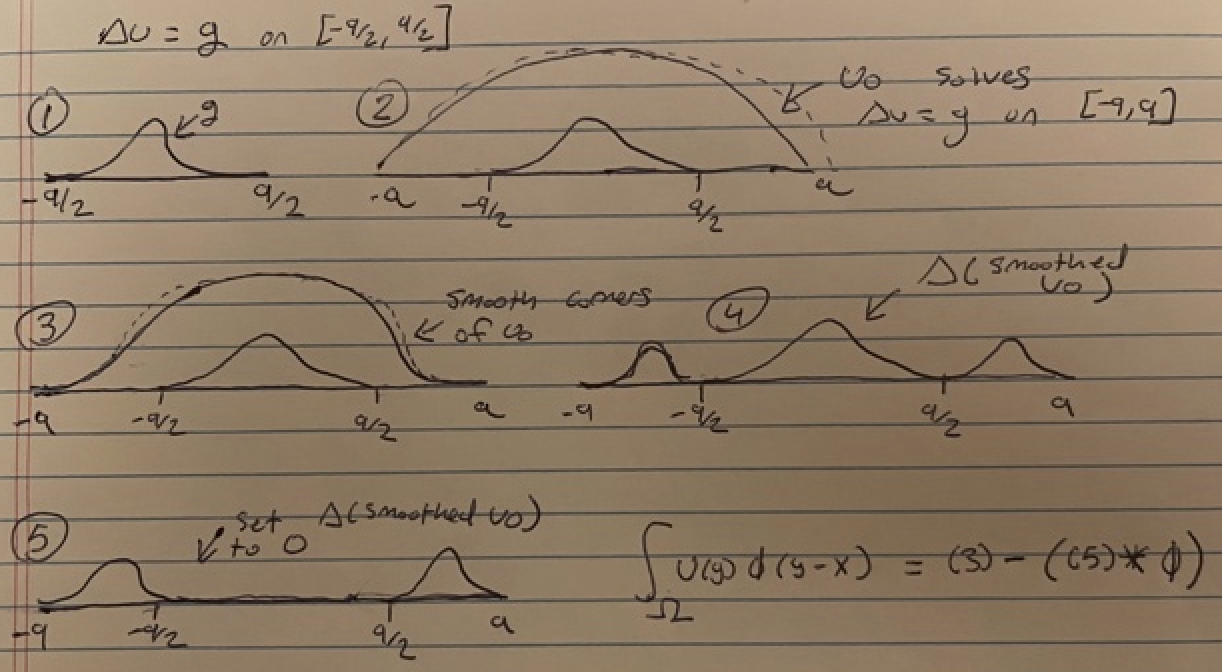
\includegraphics[scale=.5]{con_method.png}
    \caption{Convolution Method}
  \end{figure}
\end{frame}


\begin{frame}
    \frametitle{Numerical Results- Initial Conductivity}
            \centering
            \begin{figure}
            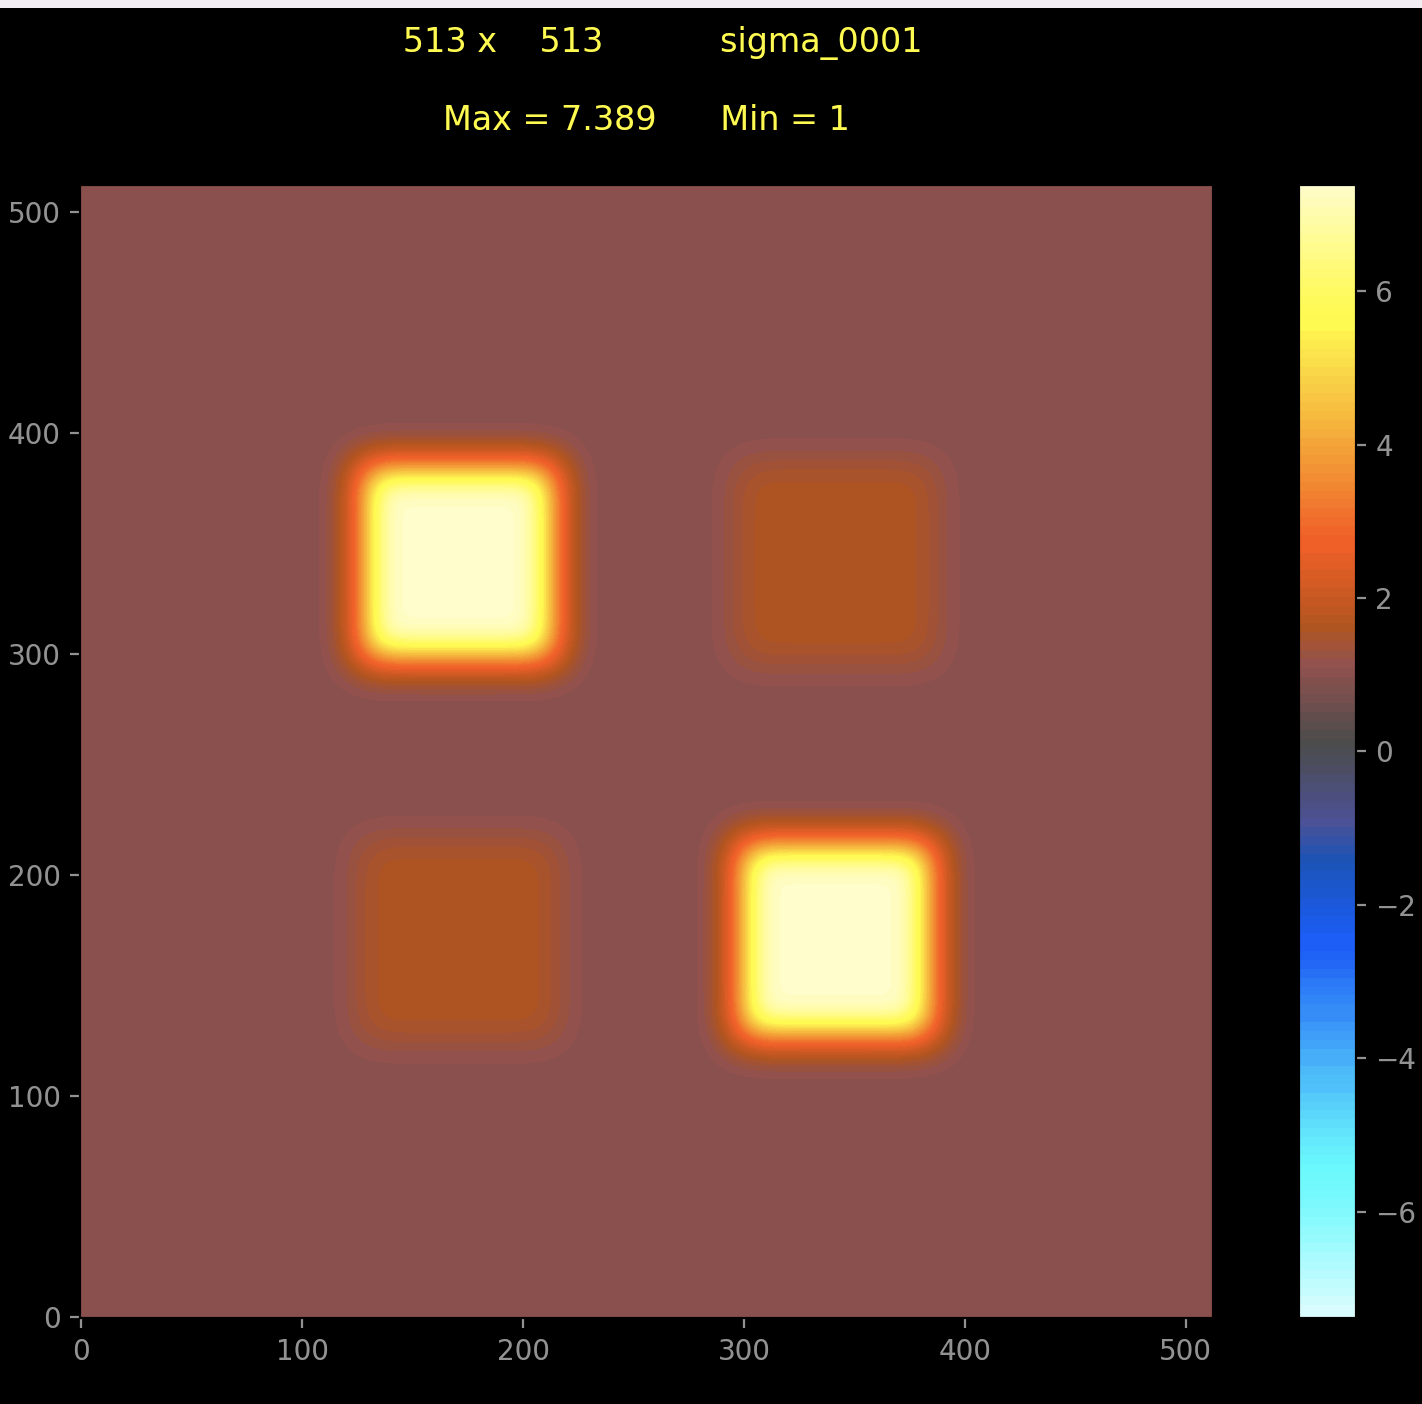
\includegraphics[scale=0.20]{sigma1.png}
            \caption{Conductivity $\sigma(x)$}
            \end{figure}
\end{frame}

\begin{frame}
    \frametitle{Numerical Results- Point Source Potential}
            \centering
            \begin{figure}
            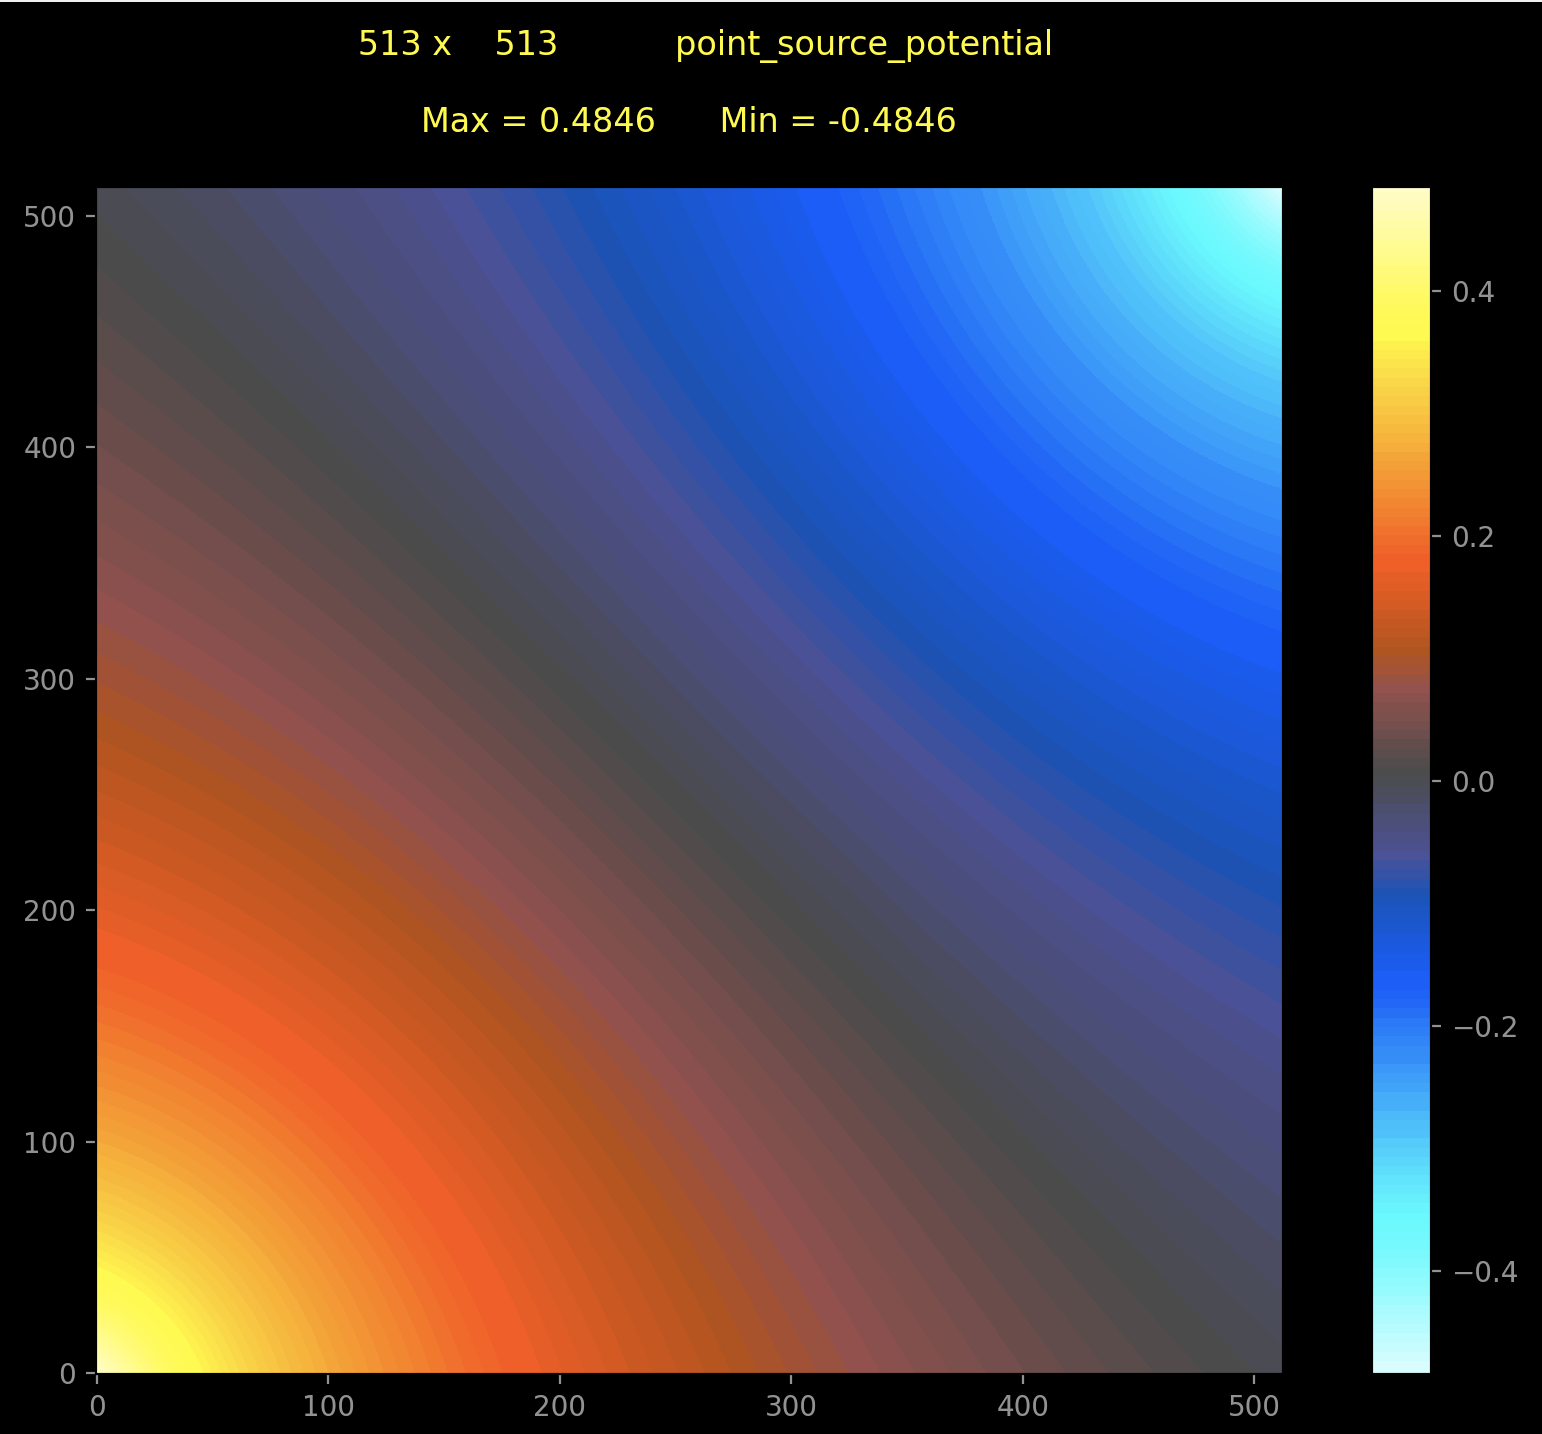
\includegraphics[scale=.20]{point_sources.png}
            \caption{Point Source Potential $w(x)$}
            \end{figure}
  \end{frame}

  \begin{frame}
      \frametitle{Numerical Results- Laplacian of Smooth Potential (GMRES output)}
            \centering
            \begin{figure}
            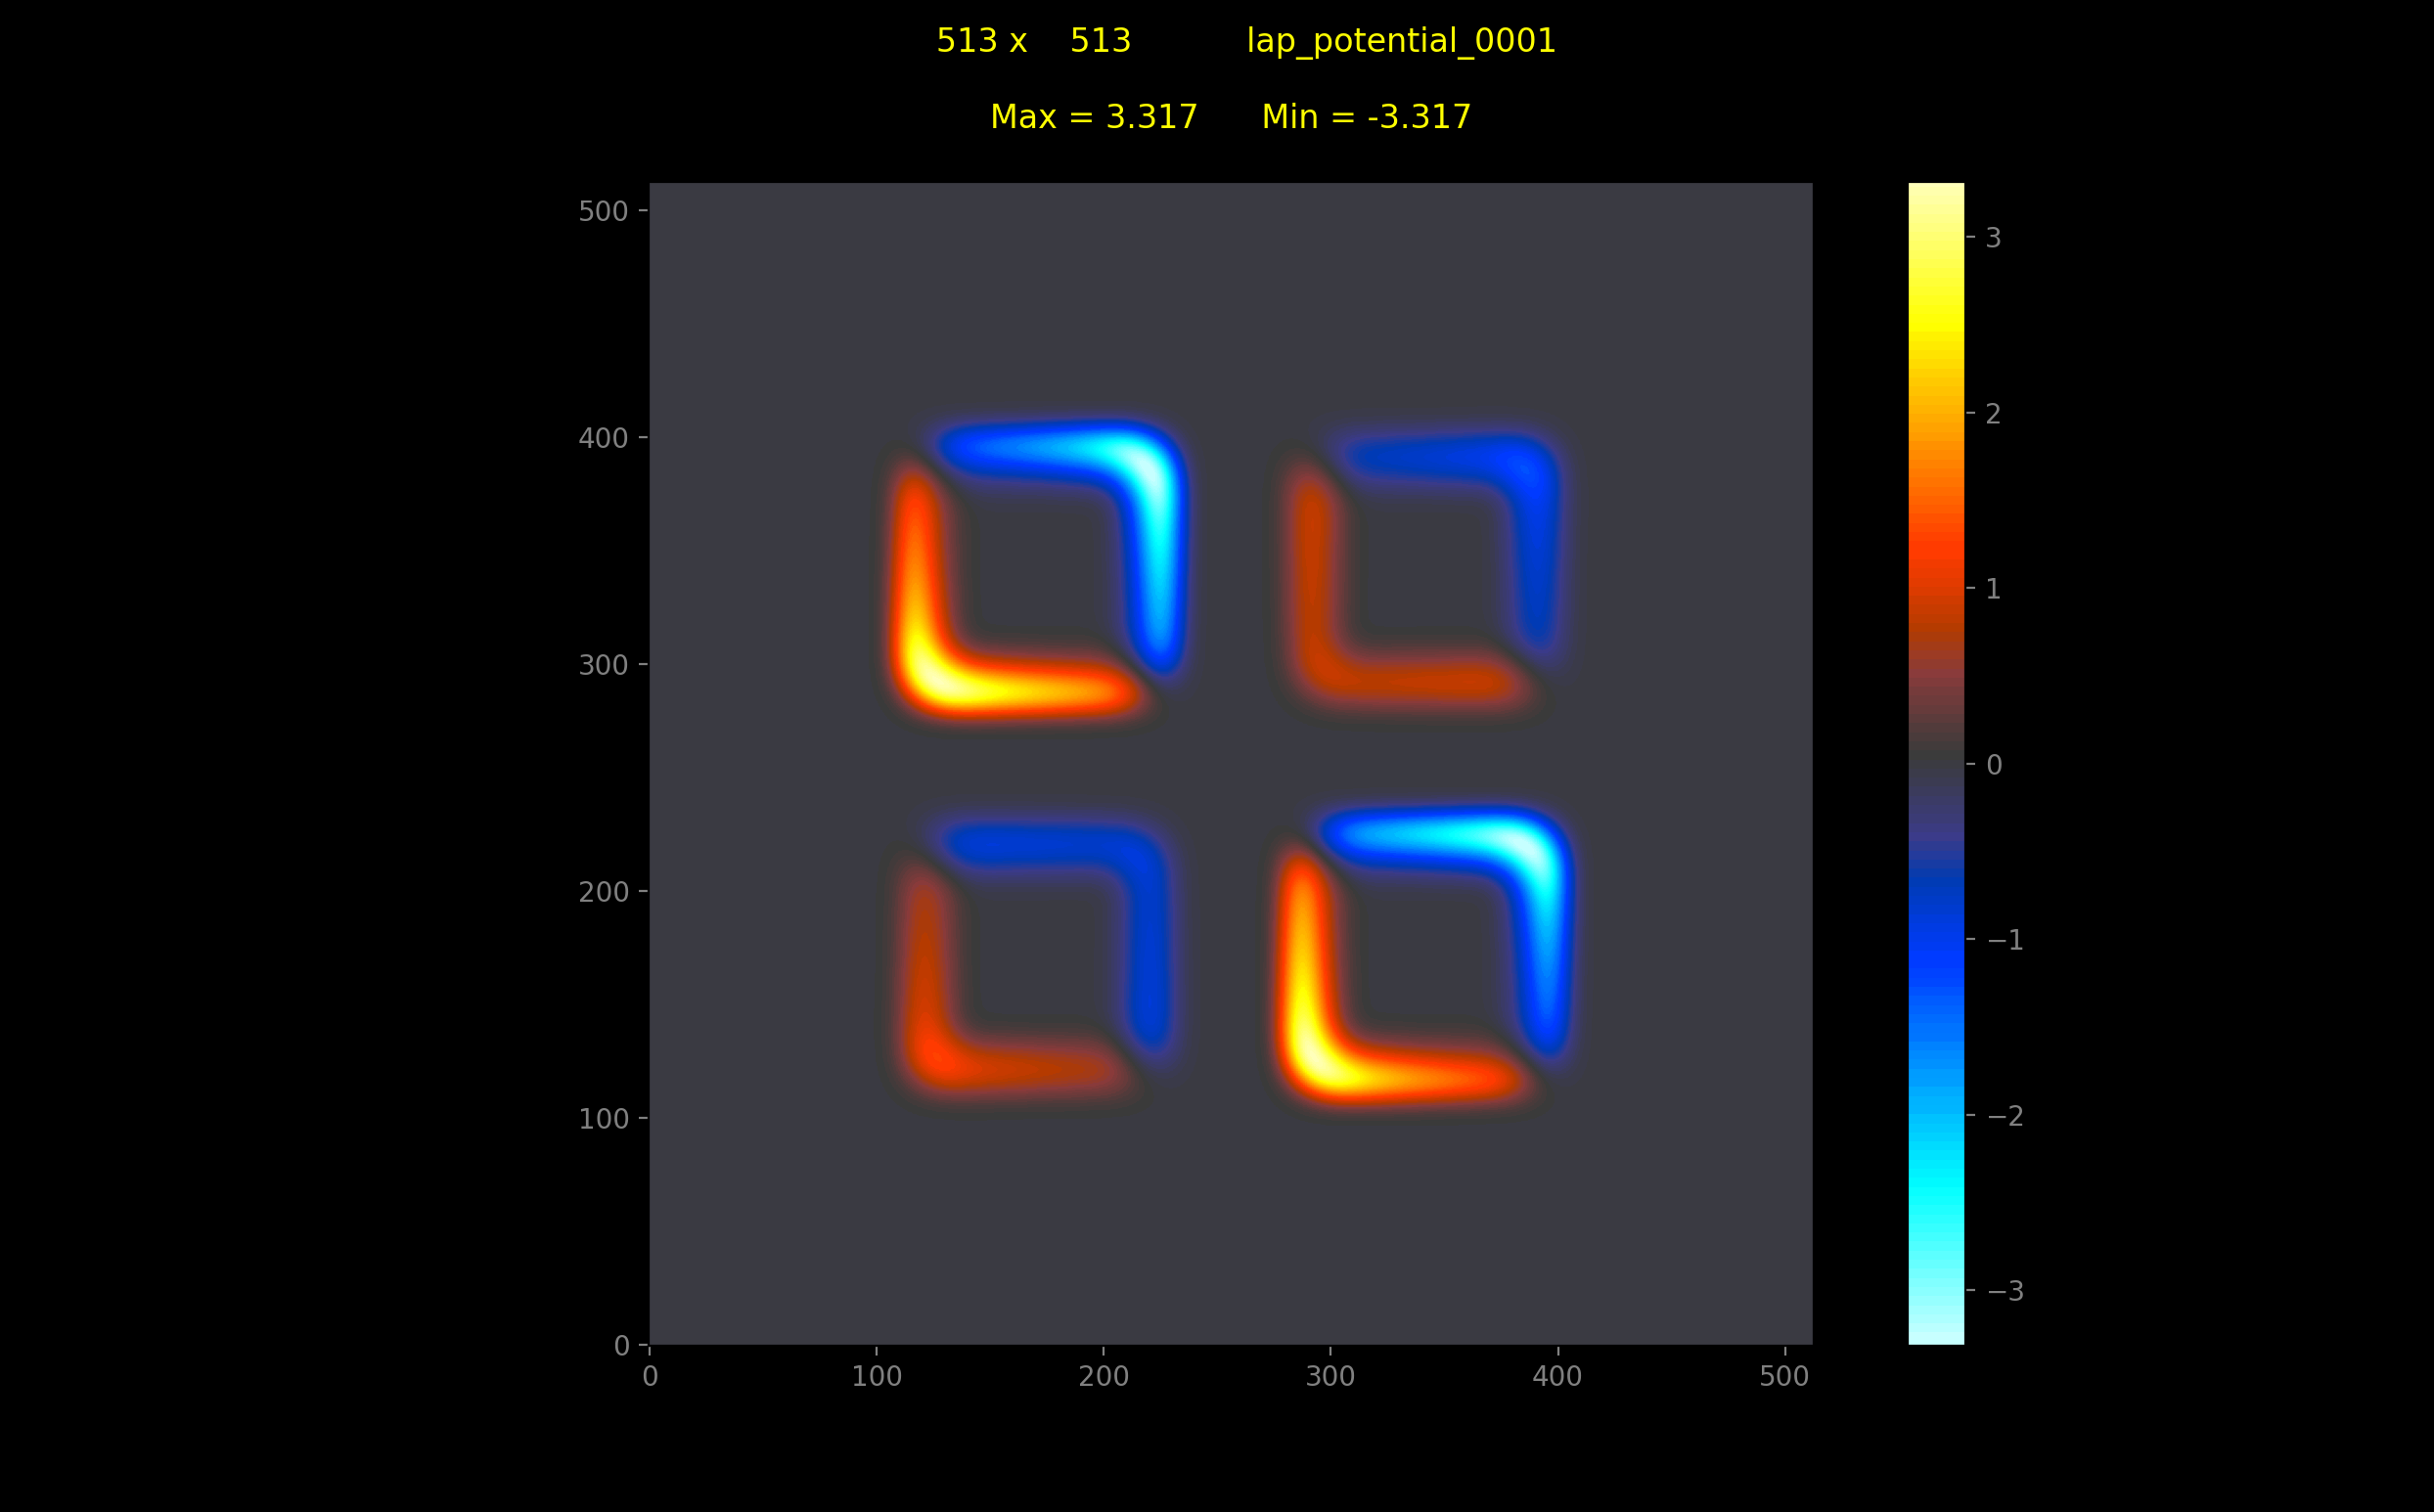
\includegraphics[scale=.20]{lap_potential.png}
            \caption{Laplacian of Smooth Potential $\Delta u(x)$}
            \end{figure}
  \end{frame}

    \begin{frame}
      \frametitle{Numerical Results- Smooth Potential}
            \centering
            \begin{figure}
            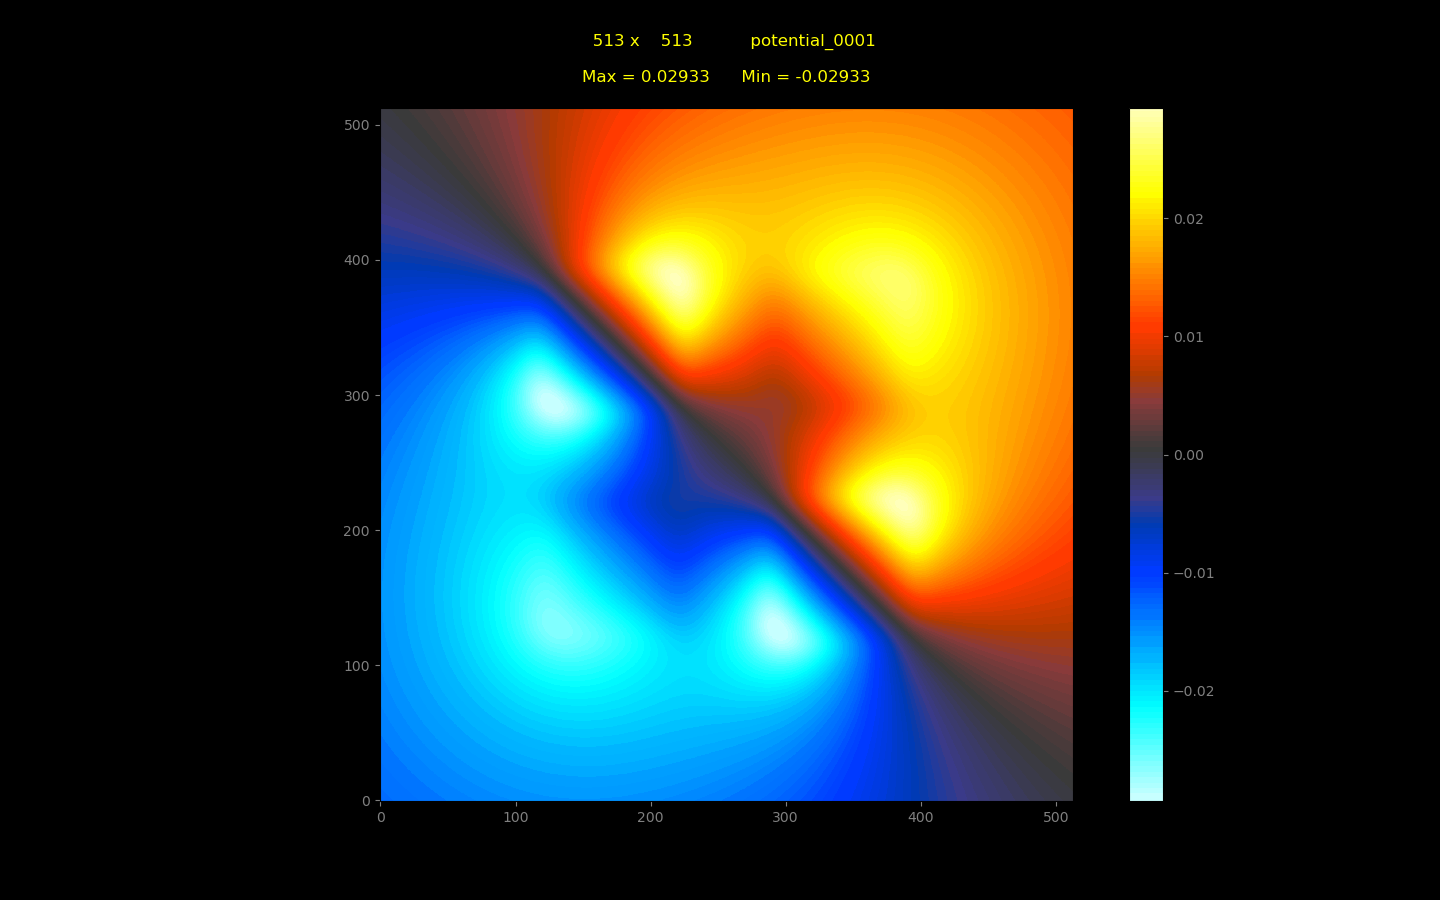
\includegraphics[scale=.20]{smooth_potential.png}
            \caption{Smooth Potential $u(x)$}
            \end{figure}
  \end{frame}

   \begin{frame}
      \frametitle{Numerical Results- GMRES Error}
            \centering
            \begin{figure}
            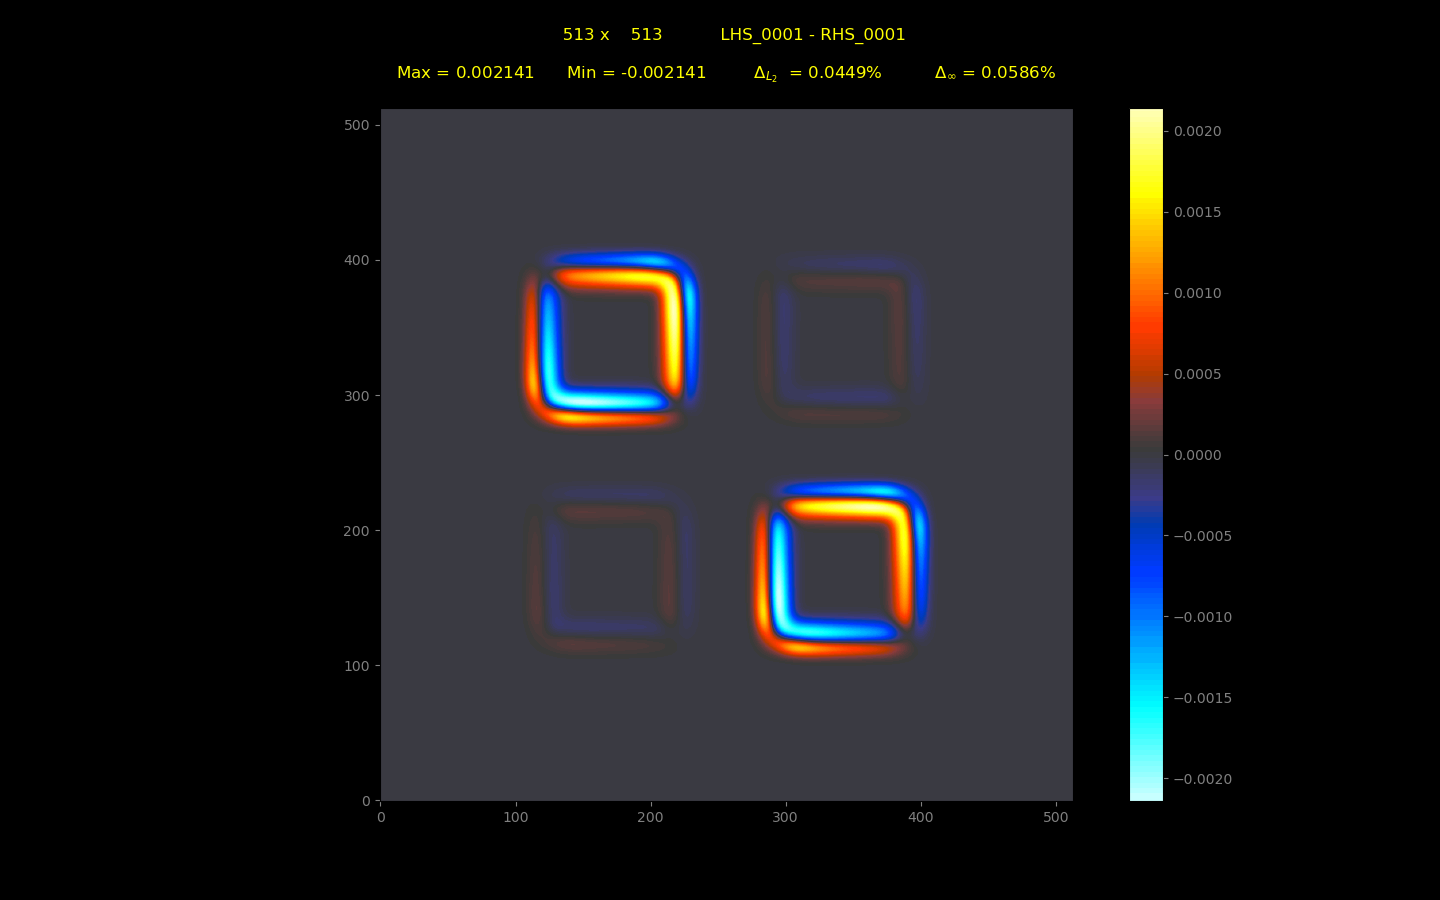
\includegraphics[scale=.20]{error.png}
            \caption{LHS v RHS Error}
            \end{figure}
  \end{frame}

   \begin{frame}
      \frametitle{Numerical Results- Curl of Lead Currents}
            \centering
            \begin{figure}
            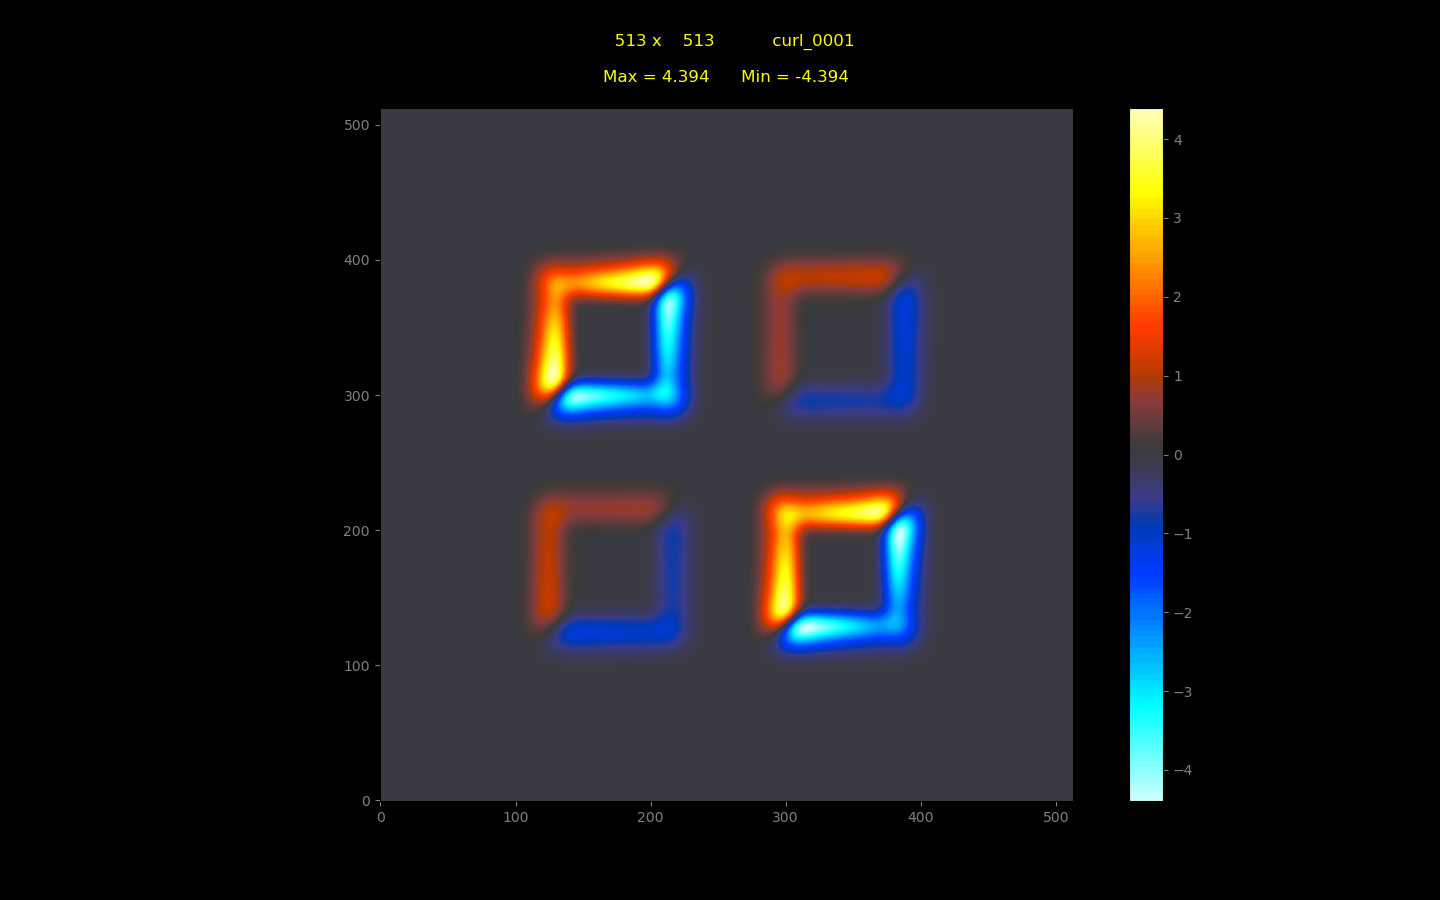
\includegraphics[scale=.20]{curl.png}
            \caption{Curl of Lead Current $\nabla \times J_{I}(x)$}
            \end{figure}
  \end{frame}

   \begin{frame}
      \frametitle{Numerical Results- Lead Currents}
            \centering
            \begin{figure}
            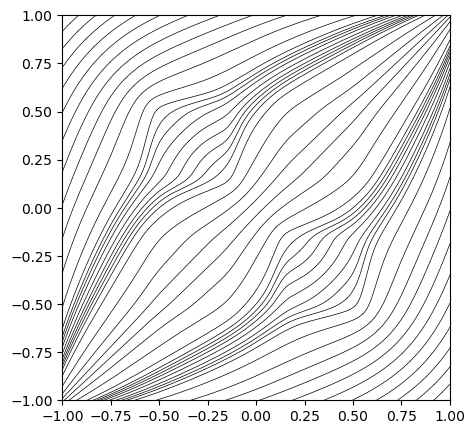
\includegraphics[scale=.40]{center_midpoint_0001.png}
            \caption{Depiction of Current Lines}
            \end{figure}
  \end{frame}












%\begin{frame}
 % \frametitle{The Problem we are Considering}
  %\begin{itemize}
   %   \item Suppose now we have a region $\Omega$, not containing any of the injection points $y^{(j)}$, where conductivity is non-constant. ie, conductivity is given by some function $\sigma(x), x \in \Omega$.
    %\item By superposition, we can split the resulting electric potential into the potential given by the injected currents, and the potential arising when conductivity is no longer constant. Then current is given by $\sigma(x)\nabla(u(x)+w(x))$.
    %\item Divergence of total current is $0$ away from the injection points, and $u(x)$ vanishes at $\infty$.
%\end{itemize}
%\end{frame}

%\begin{frame}
 % \frametitle{The Conductivity Equation - Setup}
 % \begin{figure}
  %  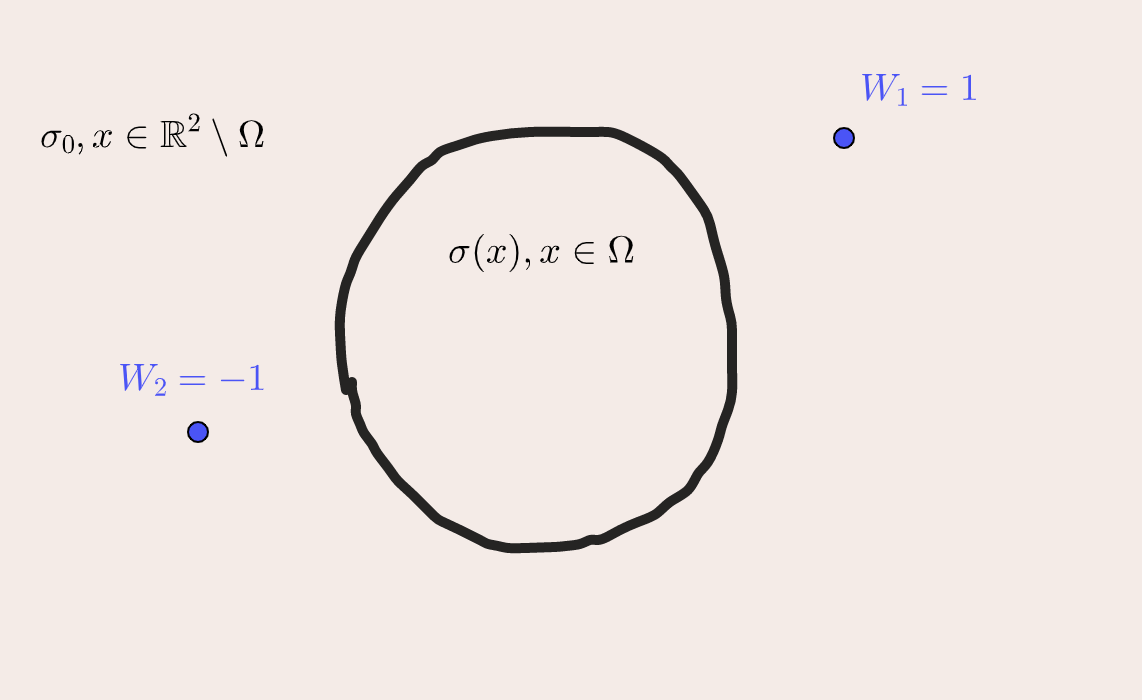
\includegraphics[scale=0.33]{cond_graph.png}
   % \caption{Basic Setup}
   % \end{figure}
  %\[
  %    \nabla \cdot \sigma(x)\nabla(u(x)+w(x))=0, \quad x \in \mathbb{R}^2 \setminus \cup_{j=1}^{n}y^{(j)}.
  %\]

%\end{frame}


%\begin{frame}
 % \frametitle{Conductivity Equation - Fredholm Reduction}
  %\begin{itemize}
   % \item For convenience, we let $U(x) = \Delta u(x)$.
   %\item It can be shown that the conductivity equation can be expressed as an integral equation of the second kind
   %     \[U(x) + \nabla \ln(\sigma(x))\cdot \nabla [\int_{\Omega}U(y)\phi(x-y)dy] = -\nabla \sigma(x)\cdot\nabla w(x), x \in \Omega.\]
    %\item Such equations are known to be well-posed.
  %\end{itemize}
%\end{frame}


%\begin{frame}
 %   \frametitle{Primary Problem- Convolution with a Singular Kernel}
 %   \begin{itemize}
 %       \item We want to make a numerical solver to reconstruct currents for arbitrary $\sigma(x)$.
 %       \item Since we are using the Fredholm Equation of the Second kind formulation, we need to handle convolutions with a singular kernel $u(x) = \int_{\Omega}U(y)\frac{1}{2\pi}\ln|y-x|dy$
 %       \item Result of the convolution will satisfy the following conditions:
  %      \item (1) $\Delta u(x) = U(x), x \in \Omega$
  %      \item (2) $\Delta u(x) = 0, x \notin \Omega$.
  %      \item (3) $u(x)$ behaves like a Logarithm asymptotically.
  %      \item A function satisfying (1)-(3) will be unique.
  %      \item For simplicity, we take $\Omega = [-a/2,a/2]^2$, but the following approach should work for any $\Omega$.
  %  \end{itemize}
%\end{frame}

%\begin{frame}
%    \frametitle{Convolution Method - Descrption}
%     Our goal is to compute $u(x) = \int_{\Omega}U(y)\frac{1}{2\pi}\ln|y-x|dy$.
%     \begin{itemize}
%        \item Step 1- Compute the solution having $0$ boundary conditions on a larger square via Sine series.
%        \item Step 2- Smoothly cutoff the corners of the resulting solution.
%        \item Step 3- Compute the laplacian of the resulting function.
%        \item Step 4- Set the laplacian to $0$ over the small square.
%        \item Step 5- Compute the convolution of the resulting with the fundamental solution, taking the convolution over the small square.
%        \item Step 6- Subtract the result of the convolution from the smoothly cutoff solution.
%    \end{itemize}
%  \end{frame}


%\begin{frame}
%    \frametitle{Convolution Method - In Pictures}
 %    \begin{figure}
 %  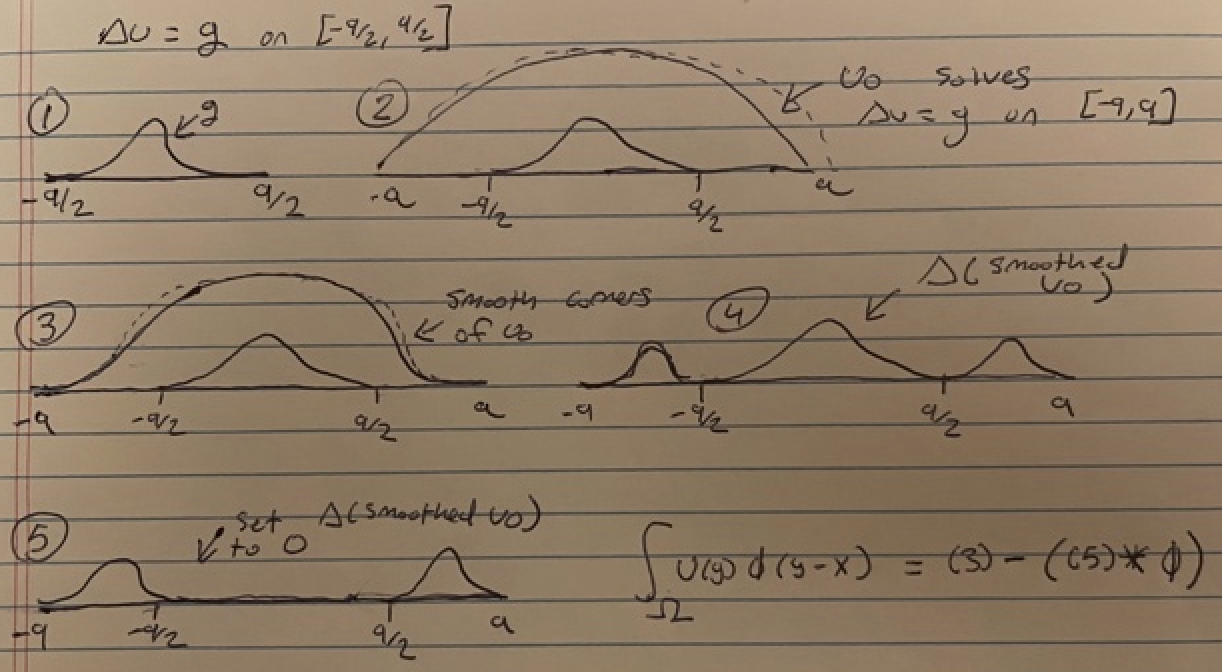
\includegraphics[scale=.5]{con_method.png}
 %   \caption{Convolution Method}
 % \end{figure}
%\end{frame}

%\begin{frame}
 %   \frametitle{Why it Works + Beneftis}
  %  \begin{itemize}
  %      \item  $\Delta u_{\text{final}}= U(x)$ inside of $\Omega$.
  %       \item $\Delta u_{\text{final}}= 0$ outside of $\Omega$.
  %      \item $u_{\text{final}}$ behaves like a logarithm asymptotically.
  %      \item Therefore, $u_{\text{final}} = \int_{\omega}U(y)\phi|y-x|$.
  %      \item We completely avoid the singularity in the kernel $\phi(x)$.
  %      \item All non-trivial computations - computing the laplacian, inverting the laplcian, taking the convolution, computing partial derivatives- can be done via FFT methods.
  %  \end{itemize}
 %\end{frame}



%\begin{frame}
 %   \frametitle{Convolution Method- Numerical Example}
  %  We test a numerical scheme using the function $(1-\hat{\sin(x)})\ln(|x|)$. This function has a laplacian which we can exactly compute, and behaves like a logarithm asymptotically.
 %\begin{figure}
  % 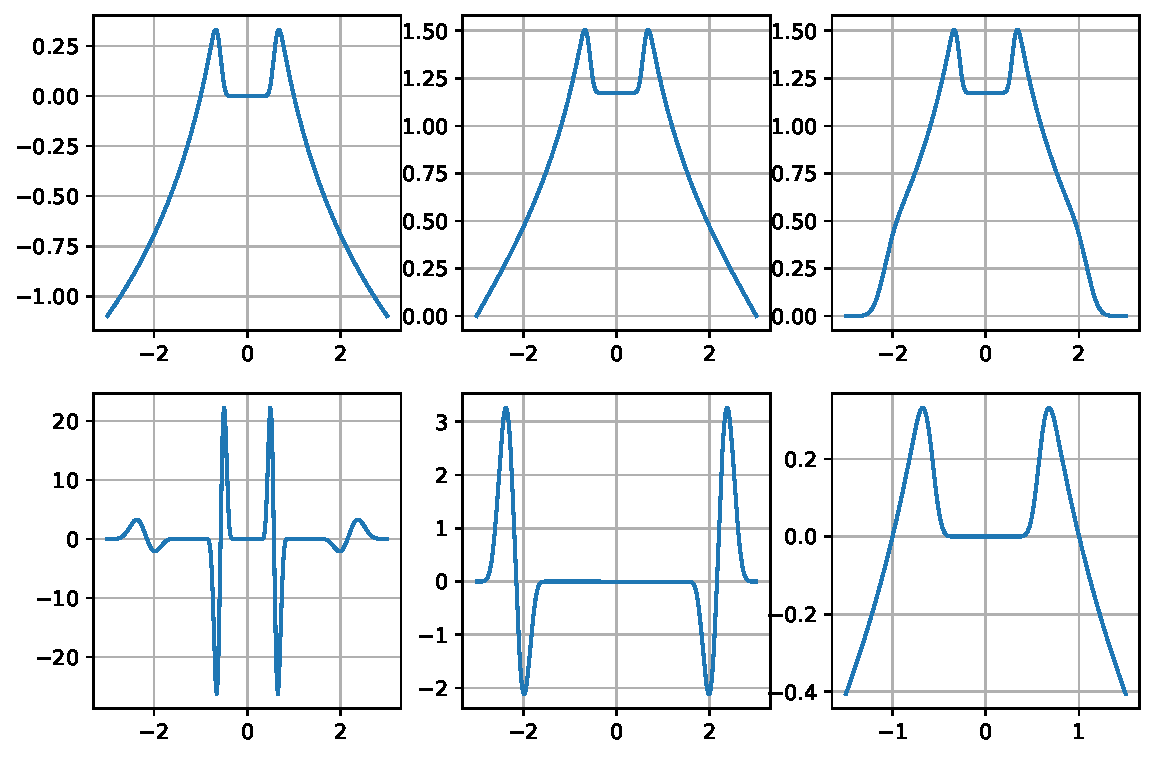
\includegraphics[scale=.3]{convolution_method.pdf}
   % \caption{Numerical Example}
%\end{figure}
%\end{frame}


%\begin{frame}
 %   \frametitle{Computing the Convolution- Error}
 %   \begin{figure}
 %   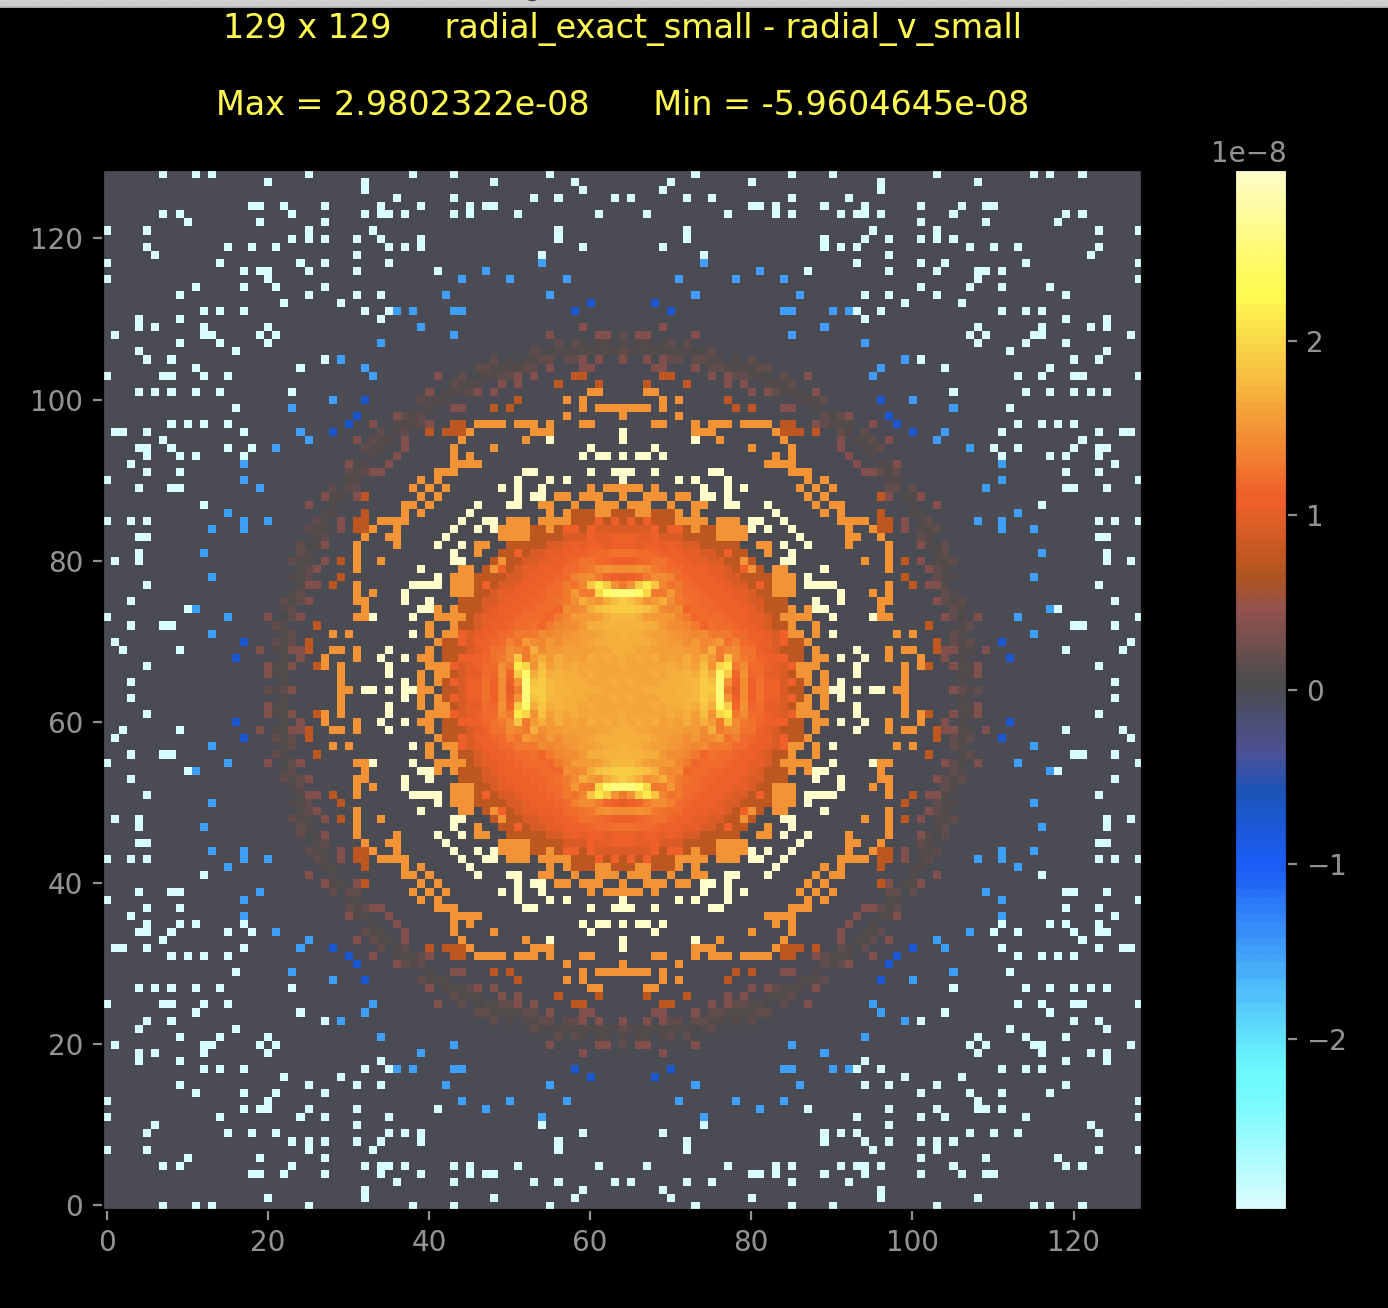
\includegraphics[scale=.25]{v_err.png}
 %   \caption{Difference between $u_{\text{final}}$ and exact solution}
 %   \end{figure}
%\end{frame}

\end{document}
